\subsection{\acrlong{lda}}\label{sec:lda}
\todo[inline]{describe goal / purpose / idea}
\Gls{lda} is topic model method. The objective of topic modeling is to infer topics (collections of words) in a document set.

\begin{definition}\label{def:topic}
	\textit{A topic is a distribution over words in a corpus.}
\end{definition}

The result consists of a topic-word distribution matrix $\beta$, which for each topic gives a distribution of words belonging to said topic, and a document-topic distribution matrix $\theta$ which for each document gives a distribution of topics to which the document belongs to.

\citeauthor{lda} \cite{lda} introduced \gls{lda}, which has since become a staple within topic modeling.
\gls{lda} works under the assumption that documents are generated from a specific generative process, and tries to reverse engineer this process.
This generative process assumes that documents are random mixtures of latent topics and that each topic is a distribution over all the words in the corpus.

This process generates $K$ topics and $D$ documents containing $N_{d}$ words, where $d$ is a document in $D$.
The generative process has two Dirichlet distributions $Dir(\alpha)$ for the document-topic relation and $Dir(\eta)$ for the topic-word relation.

\begin{figure}[h]
	\centering
	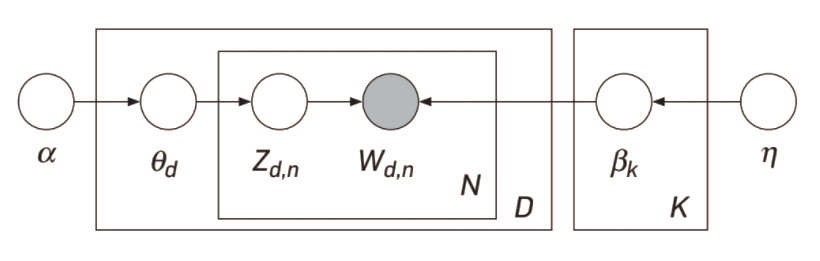
\includegraphics[width=0.5\textwidth]{figures/Smoothed_LDA.jpg}
	\caption{Plate notation for \gls{lda}. Boxes symbolize repeated processes, shaded elements are observed information. Image is from \citet{blei2012topicmodels}.}
	\label{fig:lda}
\end{figure}

From these Dirichlet distributions, we can sample two multinomial distributions: a document-topic distribution $\theta_d$ for each document $d$, and a topic-word distribution $\beta_k$ for each topic $k$.
$\theta$ and $\beta$ are stored as matrices.
These Dirichlet distributions are tuned with the hyperparameters $\alpha$ and $\eta$, which adjust the entropy of the sampled distributions.
An $\alpha$ value near 1 causes each document to be distributed over almost all topics, while an $\alpha$ value near 0 causes each document to be distributed over only a few topics.
Similarly $\eta$ will adjust how many words each topic contains.
This also has the added consequence that a high $\alpha$ will make documents appear more similar, and a high $\eta$ will make topics appear more similar.

Using $\theta$ and $\beta$, we can sample concrete topics $Z$ from documents, and concrete words $W$ from topics.
\autoref{fig:lda} gives an overview of the generative process.

\Gls{lda} has some underlying assumptions, which also explain its limitations\cite{blei2012topicmodels}:
\begin{itemize}
	\item \gls{lda} assumes ordering of words does not matter (Bag of Words).
	\item \gls{lda} assumes ordering of documents does not matter.
	\item \gls{lda} assumes that the number of topics is fixed and known.
\end{itemize}
However, many of these assumptions can be addressed through various extensions of the \gls{lda} model\cite{blei2012topicmodels}.

\subsubsection{\gls{lda}-\gls{ir}}\label{subsec:lda_ir}
\todo[inline]{describe goal / purpose / idea}
\citeauthor{yang2009topic}\cite{yang2009topic} defines \autoref{eq:lda-ir} for using \gls{lda} as an \gls{ir} method. 
They do this based on a previous application of \gls{lda} for \gls{ir}\cite{lda-ir}.

\begin{equation}\label{eq:lda-ir}
	P(w|d, \theta, \beta) = \sum_{z \in T} P(w|z,\beta_z) P(z|d,\theta_d)
\end{equation}

The idea behind this equation is to reverse-engineer the generative process \gls{lda} uses to create the topic model, to predict the probability of a word appearing in a document given the document-topic distribution matrix $\theta$ and the topic-word distribution matrix $\beta$.
We use the term \gls{lda}-\gls{ir}, to refer to information retrieval made using \autoref{eq:lda-ir}.
